\chapter{Simulation}
	To test the performance of the guidance system, it is implemented in matlab/simulink. A number of
	scenarios are used to test how it performes in various conditions.

	The proposed system are greatly simplyfied and there are a number of situations that it will not work
	well. This situations are also threated and discussed in the next chapter. 
	

\section{Matlab}
	The mathematical model of the \textit{HUGIN 1000} AUV are implemented in simulink using the
	\textit{GNC} toolbox available from \textit{www.marinecontrol.org} with slight modifications to the
	6DOF model.

	The Camera output simulator were programmed in matlab. It inputs the position of the AUV and
	transposes it to body coordinates to calculate the field of view of the camera. The camera are based
	on the pinhole camera model with unity focus distance, and a view angle of about 45 degrees. The
	program then calculates the field of view of the camera and checks if there are any part of the
	pipeline inside the field of view. The output of the camera are three points taken out at the top, the
	middle and the bottom of the field of view.

	A sonar which determines the altitude are implemented using a look-up table with a predefined bottom
	profile.

	The descision logic is implemented as a state machine, and gives out the desired heading dependent on
	what state the system is in.

	The filter was created using a m-file and global variables for the filter parameters. The filter
	parameters are as follows:
	\begin{equation}
		P_0 = \left [ \begin{matrix}
				10 & 0 & 0 & 0 \\
				0 & 10 & 0 & 0 \\
				0 & 0 & 0.1 & 0 \\
				0 & 0 & 0 & 0.1
				\end{matrix} \right] \quad
		W = 0.1 \mathbf{I}_{2x2} \quad Q = 10 \mathbf{I}_{2x2} 
	\end{equation}

	The final simulink diagram are shown in figure \ref{fig:ch3_simulink}.
	\begin{figure}[htbp]
		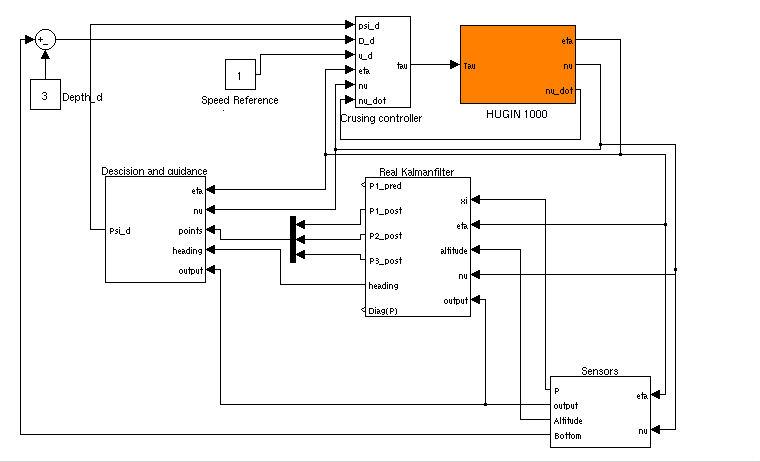
\includegraphics[width=\textwidth]{pics/simulink}
		\caption{The Simulink Diagram}
		\label{fig:ch3_simulink}
	\end{figure}

	

\section{Simulation Scenarios}
	To test the performance of the guidance system some scenarios are proposed.
	\begin{description}
		\item[\textbf{1st Scenario}.] The pipeline are at the exact location acording to predefined
		data. Environmental disturbances such as currents are turned off. The pipelien are
		continiously visible for the camera the whole inspection distance.
		\item[\textbf{2nd Scenario}.] Exact as over but with environmental forces turned on.
		\item[\textbf{3rd Scenario}.] The pipeline are at the exact location where it initially was
		layed. A section is burried, and not visible for the camera. Environmental forces are turned
		on.
		\item[\textbf{4th Scenario}.] The á priori info about the pipeline ar offset about 20 meteres
		to test the ability of the guidance system to search for the pipeline.
	\end{description}


\section{Results}
	
	


